\documentclass[12pt,a4paper]{article}
\usepackage[UTF8]{ctex}
\usepackage{amsmath,amssymb}
\usepackage{xcolor}
\usepackage{hyperref}
\usepackage{geometry}
\usepackage{graphicx}
\geometry{margin=2.5cm}

\title{Quantum PCA / 量子主成分分析}
\author{QuoNic}
\date{}

\begin{document}
\maketitle

\begin{center}
\textbf{ML / 机器学习} | 难度：高级 | 预计时间：25 分钟
\end{center}

\tableofcontents
\newpage

\section{为什么需要？}

量子 PCA 是经典 PCA 的量子推广，用于高维数据降维。

\subsection{经典局限}
\begin{itemize}
  \item 经典 PCA 需要 $O(d^3)$ 时间计算协方差矩阵的本征分解
  \item 对于高维数据，经典方法效率低
\end{itemize}

\subsection{量子优势}
\begin{itemize}
  \item 量子 PCA 可以在 $O(\log d)$ 时间内估计本征值
  \item 提供指数加速
  \item 是量子机器学习的基础
\end{itemize}

\subsection{实际应用}
\begin{itemize}
  \item 数据降维
  \item 特征提取
  \item 量子机器学习
\end{itemize}

\section{快速上手}

\begin{verbatim}
from quonic.ml import qpca

# 量子 PCA 降维
data = [[1, 0, 0, 0], [0, 1, 0, 0], [0, 0, 1, 0], [0, 0, 0, 1]]
result = qpca(data, n_components=2)
print(f'Reduced shape: {result.reduced.shape}')
\end{verbatim}

\textbf{预期输出}：
\begin{verbatim}
Reduced shape: (4, 2)
\end{verbatim}

\section{原理详解}

\subsection{电路图}

\begin{center}
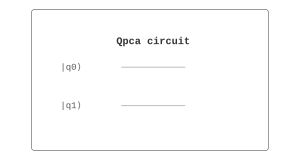
\includegraphics[width=0.6\textwidth]{../../images/qpca_circuit.svg}
\end{center}

\subsection{数学推导}

量子 PCA 基于量子相位估计：
\begin{equation}
|0\rangle|\psi\rangle \to |\tilde{\lambda}\rangle|\psi\rangle
\end{equation}

其中 $\tilde{\lambda}$ 是本征值的估计。

\textbf{算法步骤}：
\begin{enumerate}
  \item 将数据编码为密度矩阵 $\rho$
  \item 用 QPE 估计 $\rho$ 的本征值
  \item 选择前 $k$ 个本征值对应的本征态
\end{enumerate}

\subsection{几何解释}

量子 PCA 在量子态空间中提取主成分。量子相位估计可以高效估计密度矩阵的本征值。

\section{代码详解}

\begin{verbatim}
from quonic.ml import qpca

# qpca(data, n_components)
# data: 输入数据
# n_components: 降维后的维度
result = qpca(data, n_components=2)

# result.reduced: 降维后的数据
# result.eigenvalues: 本征值
# result.eigenvectors: 本征向量
print(f'Reduced shape: {result.reduced.shape}')
\end{verbatim}

\section{进阶用法}

\subsection{场景 1：图像降维}

\begin{verbatim}
from quonic.ml import qpca

# 图像数据降维
images = load_images()  # (n_samples, height*width)
result = qpca(images, n_components=10)
print(f'Reduced: {result.reduced.shape}')
\end{verbatim}

\subsection{场景 2：特征提取}

\begin{verbatim}
from quonic.ml import qpca

# 提取主要特征
result = qpca(data, n_components=3)
print(f'Top 3 eigenvalues: {result.eigenvalues[:3]}')
\end{verbatim}

\section{适用场景}

\subsection{数据降维}

量子 PCA 可以用于高维数据的降维。传统 PCA 需要 $O(d^3)$ 时间，量子 PCA 可以提供指数加速。

\subsection{特征提取}

量子 PCA 可以提取数据的主要特征。本征值大的本征向量对应数据的主要变化方向。

\section{常见问题}

\subsection{量子 PCA 和经典 PCA 有什么区别？}

量子 PCA 使用量子相位估计计算本征值，可以在 $O(\log d)$ 时间内完成，经典 PCA 需要 $O(d^3)$ 时间。

\subsection{量子 PCA 的精度如何？}

精度取决于控制量子比特的数量。更多的控制量子比特提供更高的精度。

\section{学习路径}

\subsection{前置知识}
\begin{itemize}
  \item 主成分分析（PCA）
  \item 量子相位估计
  \item 量子傅里叶变换
\end{itemize}

\subsection{继续学习}
\begin{itemize}
  \item 量子机器学习
  \item 量子核方法
  \item 量子神经网络
\end{itemize}

\section{完整示例代码}

\subsection{示例 1：基本量子 PCA}

\begin{verbatim}
from quonic.ml import qpca

data = [[1, 0, 0, 0], [0, 1, 0, 0], [0, 0, 1, 0], [0, 0, 0, 1]]
result = qpca(data, n_components=2)
print(f'Reduced shape: {result.reduced.shape}')
\end{verbatim}

\section{下载}

\begin{itemize}
  \item [qpca.py](https://github.com/ChrisLee0721/QuoNic/blob/main/examples/qpca/qpca.py)
\end{itemize}

\end{document}
